
\tikzstyle{vertex} = [draw=black,circle,inner sep=0pt,minimum size=20pt]
\tikzstyle{treeedge} = [draw=green,line width=5pt]
\tikzstyle{edge} = [draw=black]
\tikzstyle{root} = [fill=red]

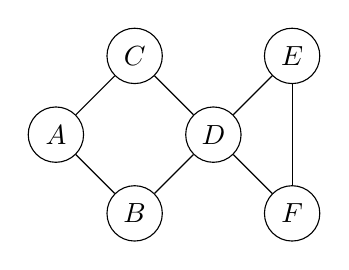
\begin{tikzpicture}
    \coordinate (A) at (0, 1);
    \coordinate (B) at (1, 0);
    \coordinate (C) at (1, 2);
    \coordinate (D) at (2, 1);
    \coordinate (E) at (3, 2);
    \coordinate (F) at (3, 0);

    \node [style=vertex] (A) at (A) {$A$};
    \node [style=vertex] (B) at (B) {$B$};
    \node [style=vertex] (C) at (C) {$C$};
    \node [style=vertex] (D) at (D) {$D$};
    \node [style=vertex] (E) at (E) {$E$};
    \node [style=vertex] (F) at (F) {$F$};

    \draw [style=edge] (A) -- (B);
    \draw [style=edge] (A) -- (C);
    \draw [style=edge] (B) -- (D);
    \draw [style=edge] (C) -- (D);
    \draw [style=edge] (D) -- (E);
    \draw [style=edge] (D) -- (F);
    \draw [style=edge] (E) -- (F);
\end{tikzpicture}

% \vspace{.5cm}
\onslide<2->{\begin{tikzpicture}
    % This is an invisible rectangle which draw the picture to avoid nodes to move when appear/disappear.
    \path (-1.5, 0) -- (-1.5, 4) -- (3, 4) -- (3, 0);

    \coordinate (A) at (0, .5);
    \coordinate (B) at (0, 1.75);
    \coordinate (C) at (1, 3.75);
    \coordinate (D) at (1, 2.5);
    \coordinate (E) at (2, 1.75);
    \coordinate (F) at (2, .5);

    \node [style=vertex] (A) at (A) {\only<3->{$A$}};
    \node [style=vertex] (B) at (B) {\only<3->{$B$}};
    \node [style=vertex,style=root] (C) at (C) {\only<3->{$C$}};
    \node [style=vertex] (D) at (D) {\only<3-4,6->{$D$}\only<5>{$F$}};
    \node [style=vertex] (E) at (E) {\only<3->{$E$}};
    \node [style=vertex] (F) at (F) {\only<3-4,6->{$F$}\only<5>{$D$}};

    \draw [style=treeedge] (A) -- (B);
    \draw [style=treeedge] (B) -- (D);
    \draw [style=treeedge] (C) -- (D);
    \draw [style=treeedge] (D) -- (E);
    \draw [style=treeedge] (E) -- (F);

    \draw<4-> [style=edge] (A) -- (B);
    \draw<4-> [style=edge] (A) .. controls (-1.2,2.5) and (0,1.5) .. (C);
    \draw<4,6-> [style=edge] (B) -- (D);
    \draw<4,6-> [style=edge] (C) -- (D);
    \draw<4-> [style=edge] (D) -- (E);
    \draw<4-> [style=edge] (D) .. controls (1.7,1.3) and (1.5,.8) .. (F);
    \draw<4-> [style=edge] (E) -- (F);

    \draw<5> [style=edge,draw=red,ultra thick] (B) .. controls (1,.5) and (1.5,.5) .. (F);
    \draw<5> [style=edge] (C) .. controls (1.75,2) and (3,2.5) .. (F);
\end{tikzpicture}}
\onslide<6->{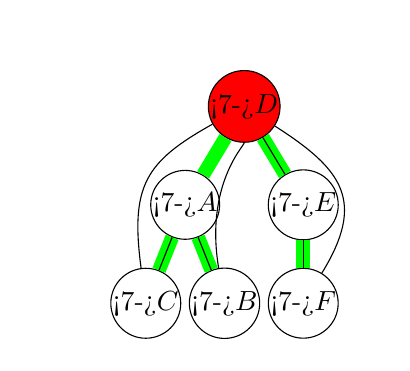
\begin{tikzpicture}
    % This is an invisible rectangle which draw the picture to avoid nodes to move when appear/disappear.
    \path (-1.5, 0) -- (-1.5, 4) -- (3, 4) -- (3, 0);

    \coordinate (A) at (.5, 1.75);
    \coordinate (B) at (1, .5);
    \coordinate (C) at (0, .5);
    \coordinate (D) at (1.25, 3);
    \coordinate (E) at (2, 1.75);
    \coordinate (F) at (2, .5);

    \node [style=vertex] (A) at (A) {\only<7->{$A$}};
    \node [style=vertex] (B) at (B) {\only<7->{$B$}};
    \node [style=vertex] (C) at (C) {\only<7->{$C$}};
    \node [style=vertex,style=root] (D) at (D) {\only<7->{$D$}};
    \node [style=vertex] (E) at (E) {\only<7->{$E$}};
    \node [style=vertex] (F) at (F) {\only<7->{$F$}};

    \draw [style=treeedge] (A) -- (B);
    \draw [style=treeedge] (A) -- (C);
    \draw [style=treeedge] (A) -- (D);
    \draw [style=treeedge] (D) -- (E);
    \draw [style=treeedge] (E) -- (F);

    \draw<8-> [style=edge] (A) -- (B);
    \draw<8-> [style=edge] (A) -- (C);
    \draw<8-> [style=edge] (B) .. controls (.75,2) and (1.25,2.5) .. (D);
    \draw<8-> [style=edge] (C) .. controls (-.2,2) and (0,2.3) .. (D);
    \draw<8-> [style=edge] (D) -- (E);
    \draw<8-> [style=edge] (D) .. controls (2.5,2.2) and (2.8,1.8) .. (F);
    \draw<8-> [style=edge] (E) -- (F);
\end{tikzpicture}}